\chapter{GIỚI THIỆU CHUNG} \label{chap:intro}

Chương này trình bày về tổng quan

\section{Lịch sử nghiên cứu}

\begin{figure}[ht]
      \centering
      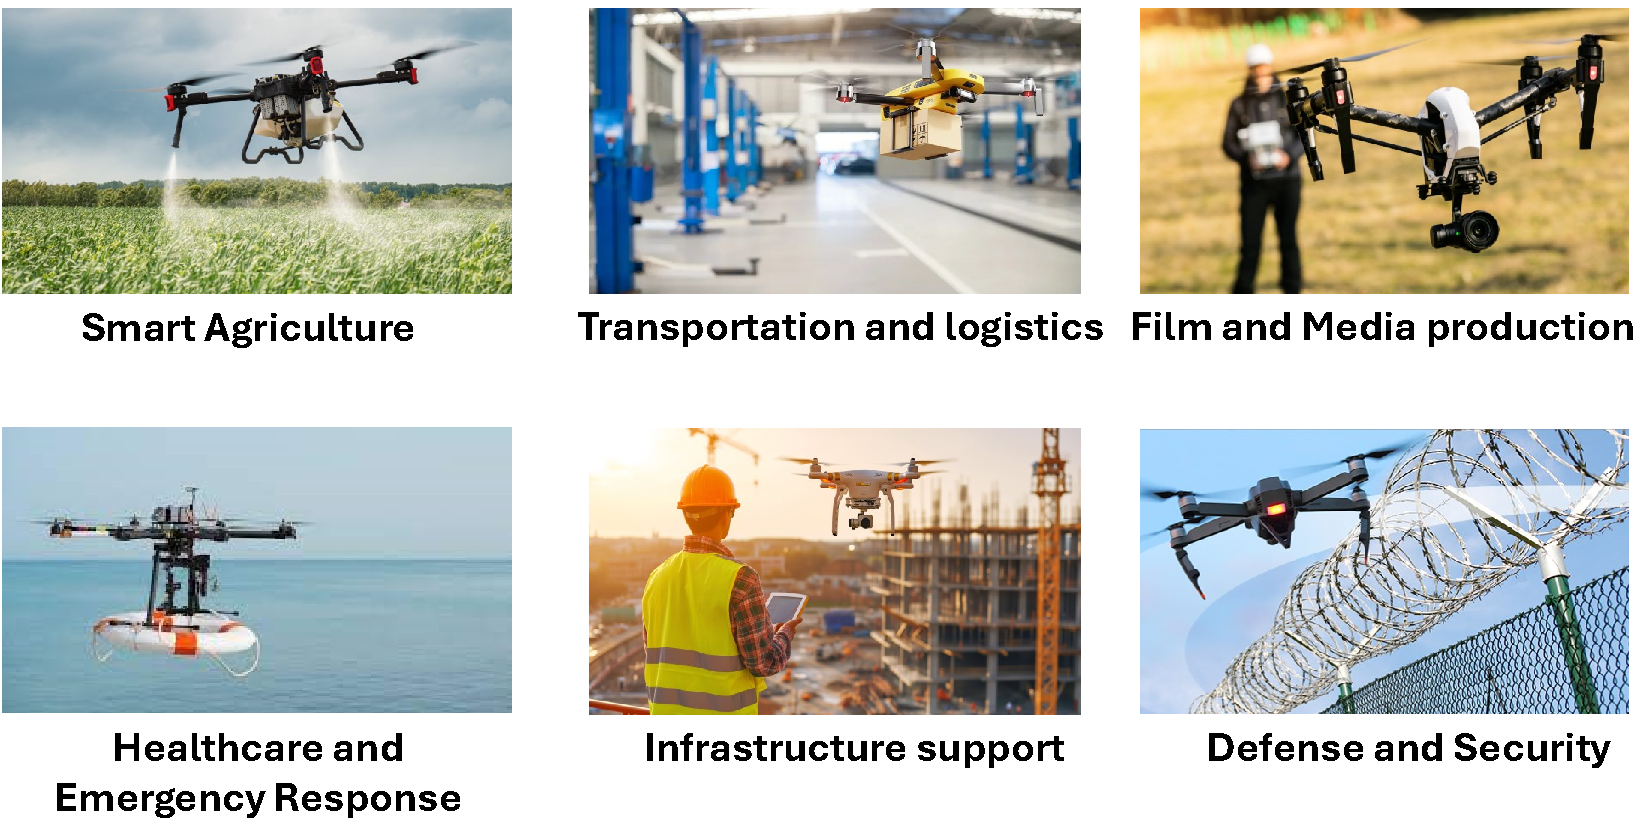
\includegraphics[scale=0.53]{Figures/drone application.pdf}
      \caption{Ứng dụng công nghệ robot trong sản xuất}
      \label{fig: drone application}
\end{figure}

Trong bối cảnh công nghiệp 4.0 đang phát triển mạnh mẽ, việc tự động hóa các khâu sản xuất và kiểm tra sản phẩm trong ngành điện – điện tử ngày càng được quan tâm. Trước đây, việc kiểm tra linh kiện mạch điện tử chủ yếu được thực hiện thủ công bởi con người, phụ thuộc vào kinh nghiệm và độ chính xác của kỹ thuật viên. Tuy nhiên, phương pháp này tốn nhiều thời gian, dễ sai sót và khó đáp ứng yêu cầu sản xuất hàng loạt với độ chính xác cao. Chính vì vậy, các hướng nghiên cứu về tự động hóa kiểm tra linh kiện đã được hình thành từ sớm, đặc biệt là trong lĩnh vực robot công nghiệp và xử lý ảnh máy tính.

Từ những năm 1990, các robot công nghiệp đã được sử dụng rộng rãi trong dây chuyền sản xuất linh kiện điện tử tại Nhật Bản, Hàn Quốc và Đức. Ban đầu, robot chủ yếu đảm nhiệm thao tác gắp – đặt linh kiện (pick and place) với độ chính xác cao, nhưng khả năng “nhận biết” linh kiện vẫn còn hạn chế do chưa có sự kết hợp với thị giác máy tính. Đến giai đoạn 2010 trở lại đây, cùng với sự phát triển của camera công nghiệp, thị giác máy tính (computer vision) và trí tuệ nhân tạo (AI), các hệ thống robot đã được nâng cấp để có thể phát hiện, nhận dạng và phân loại linh kiện một cách tự động.


\section{Đối tượng và phạm vi nghiên cứu}

\subsection{Đối tượng nghiên cứu}

Đối tượng mà đề tài nhóm tập trung nghiên cứu là mạch nguồn ổn áp tuyến tính, trong đó xem xét hai trạng thái chính: mạch đã lắp đầy đủ linh kiện và mạch bị thiếu một hoặc nhiều linh kiện. Việc lựa chọn lỗi thiếu linh kiện làm trọng tâm là do đây là dạng lỗi thường xảy ra trong quá trình sản xuất và có thể ảnh hưởng nghiêm trọng đến hoạt động ổn định của thiết bị. Thông qua hệ thống sử dụng camera và xử lý ảnh, kết hợp với tay máy robot và PLC, hình ảnh của các bo mạch sẽ được thu thập, phân tích và phân loại nhằm phát hiện sự thiếu hụt linh kiện. Mục tiêu là xây dựng một hệ thống kiểm tra tự động, có khả năng phát hiện lỗi thiếu linh kiện trên mạch nguồn ổn áp tuyến tính với độ chính xác cao, từ đó nâng cao hiệu quả kiểm tra và đảm bảo chất lượng sản phẩm đầu ra.

\section{Cấu trúc báo cáo}

Bài báo cáo bao gồm các nội dung sau:

\begin{itemize}
    \item Chương \hyperref[chap:intro]{1} Giới thiệu chung về các nội dung liên quan đến đề tài.

    \item Chương \hyperref[chap:background]{2} cơ sở lý thuyết để giới thiệu các thiết bị sử dụng trong mô hình.

    \item Chương \hyperref[chap:tombo-L1]{3} tính toán, thiết kế và chế tạo.

    \item Chương \hyperref[chap:tombo-encoder]{4} chế tạo mô hình và đánh giá.

    \item Chương \hyperref[chap:conclusion]{5} tổng kết và hướng nghiên cứu tương lai.
\end{itemize}
